\begin{figure}
    \centering
    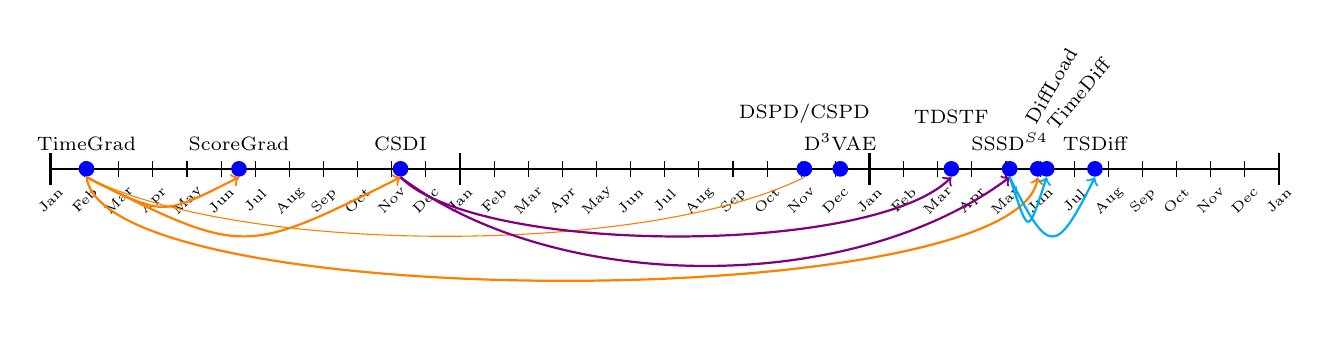
\begin{tikzpicture}[every label/.style={font=\scriptsize}]
        % Define a scale factor for years and start year
        \def\years{3}
        \def\months{\numexpr\years*12}
        \def\yearscale{5.2}
        \def\startyear{2021}
        \def\monthnames{{"Jan", "Feb", "Mar", "Apr", "May", "Jun", "Jul", "Aug", "Sep", "Oct", "Nov", "Dec"}}
    
        % Drawing the basic timeline
        \draw[thick] (0,0) -- (\years*\yearscale,0); % years from starting year to the end year inclusive
    
        % Monthly ticks, month names and yearly labels
        \foreach \x in {0,1,...,\months} { % months in the given years
            \pgfmathtruncatemacro\modresult{mod(\x,12)}
    
            \draw (\x/12*\yearscale,-0.1) -- (\x/12*\yearscale,0.1);
        
            \node[below, rotate=45, inner sep=2pt, font=\tiny] at (\x/12*\yearscale-0.1,-0.3) {\pgfmathparse{\monthnames[Mod(\x,12)]}\pgfmathresult};
            
            % Labeling years dynamically
            \tikzmath{
                int \currentYear;
                \currentYear = \startyear + div(\x,12);
            }
            \ifnum\modresult = 0
                \node[below] at (\x/12*\yearscale,1.8) {\currentYear};
                \draw[thick] (\x/12*\yearscale,-0.2) -- (\x/12*\yearscale,0.2);
            \fi
        }
    
        % Adding nodes for papers
        \node[fill=blue, circle, inner sep=2pt, label=above:{TimeGrad}, name=TimeGrad] at (32/365*\yearscale, 0) {};
        \node[fill=blue, circle, inner sep=2pt, label=above:{ScoreGrad}, name=ScoreGrad] at (168/365*\yearscale, 0) {}; 
        \node[fill=blue, circle, inner sep=2pt, label=above:{CSDI}, name=CSDI] at (312/365*\yearscale, 0) {};
        \node[fill=blue, circle, inner sep=2pt, label={[yshift=1em]above:{DSPD/CSPD}}, name=DSPD_CSPD] at (672/365*\yearscale, 0) {};
        \node[fill=blue, circle, inner sep=2pt, label=above:{D$^3$VAE}, name=D3VAE] at (704/365*\yearscale, 0) {}; 
        \node[fill=blue, circle, inner sep=2pt, label={[yshift=1em]above:{TDSTF}}, name=TDSTF] at (803/365*\yearscale, 0) {}; 
        \node[fill=blue, circle, inner sep=2pt, label=above:{SSSD$^{S4}$}, name=SSSDS4] at (855/365*\yearscale, 0) {}; 
        \node[fill=blue, circle, inner sep=2pt, label={[yshift=2.4em, xshift=1em, rotate=60]above:{DiffLoad}}, name=DiffLoad] at (880/365*\yearscale, 0) {}; 
        \node[fill=blue, circle, inner sep=2pt, label={[yshift=2em, xshift=1.6em, rotate=50]above:{TimeDiff}}, name=TimeDiff] at (888/365*\yearscale, 0) {}; 
        \node[fill=blue, circle, inner sep=2pt, label=above:{TSDiff}, name=TSDiff] at (931/365*\yearscale, 0) {}; 
    
        % Connecting papers with lines
        \draw[orange, thick, ->] (TimeGrad.south) .. controls +(1,-0.5) and +(-1,-0.5) .. (ScoreGrad.south);
        \draw[orange, thick, ->] (TimeGrad.south) .. controls +(2,-1) and +(-2,-1) .. (CSDI.south);
        \draw[orange] (TimeGrad.south) .. controls +(2,-1) and +(-2,-1) .. (DSPD_CSPD.south);
        \draw[violet, thick, ->] (CSDI.south) .. controls +(1,-1) and +(-1,-1) .. (TDSTF.south);
        \draw[violet, thick, ->] (CSDI.south) .. controls +(2,-1.5) and +(-2,-1.5) .. (SSSDS4.south);
        \draw[orange, thick, ->] (TimeGrad.south) .. controls +(0.25,-1.75) and +(-0.25,-1.75) .. (DiffLoad.south);
        \draw[cyan, thick, ->] (SSSDS4.south) .. controls +(0.25,-0.75) and +(-0.25,-0.75) .. (TimeDiff.south);
        \draw[cyan, thick, ->] (SSSDS4.south) .. controls +(0.5,-1) and +(-0.5,-1) .. (TSDiff.south);
    \end{tikzpicture}
        \caption{Diffusion for Time-series Forecasting Research Timeline}
    \label{fig:diffusion_history_time-series}
\end{figure}